\documentclass[]{article}

\begin{document}

\title{Title}
\author{Author}
\date{Today}
\maketitle

Using todays technology, generalisation of PC data upon request from the user I feasible. A proposed technical setup is described in \cite{OkholmRask******* Techpaper}.

apply tolerance, By looking at normalised data of the variance of products of the same material and process, it is possible to find a suitable tolerance
improvement per rework
material selection

\emph{What you measure and index is what you can analyse from.}
The index and type of samples limits the possible conclusions, which can be mades when extracting the data.  (If the goal is to understand the long term process capability impact of an injection mould process it is either necessary to have measurement sets from many products at different stages of their lifespan or multiple measurements through the lifespan of a couple of products.   

Initiating PCG is a tough process. 
The reward for doing robust design engineering is long reach
The reward for using PCDB or robust design in general to make changes in early design is a long term and might only benefit the company and not feedback to the designers compared the reward for the hero in production solving the expensive errors in design.

Implementing GPC requires a change
	economical barrier
		big company
			incement from quality department
			gain: 	knowledge of own PC
					high precision data
					Extensive knowledge on causes and problem
			Loss:
		cross companies
			diverse data
			gain:		Alot of data
					knowledge of processes and material outside your field
					knowledge of possible to achieve in industry
					Index storing of own data and partially analysed
			loss:		Industry espionage concerns
					loss of information due to anonymity

proto running at a university, unbiased.


ITG
Concentricity
Ca (bias,std)
Cp
circularity

ITG .. batch
ITG .. dimensions
ITG .. mold
ITG .. mold lines
ITG .. Material
ITG .. inside/outside

Ca .. radii vs. postions
Ca .. mold lines

circ .. dimension
circ .. inside/outside

conc .. dimension

ITG .. ITG spec

bias .. std

measurement tech

tol .. dimension (ISO vs. DATA)







The confidence interval of the population standard deviation is greatly effected by the sample size.  The confidence limits are given by

\begin{equation}
\left[ \sqrt{\frac{(n-1) \hat{\sigma}^2 }{\chi^2_{\alpha/2,n-1}}},  \sqrt{\frac{(n-1) \hat{\sigma}^2 }{\chi^2_{1-\alpha/2,n-1}}} \  \right]
\end{equation}
where $\chi^2$ is the chi-squared distribution, n is sample size and $\alpha$ is the significance level. The confidence limits are shown in Figure \ref{fig:std_uncertainty}. Even for samples sizes of 30 there still exist a quite large uncertainty of the standard deviation, which also directly effect the process capability indices and the calculated PCSL. 

\begin{figure}
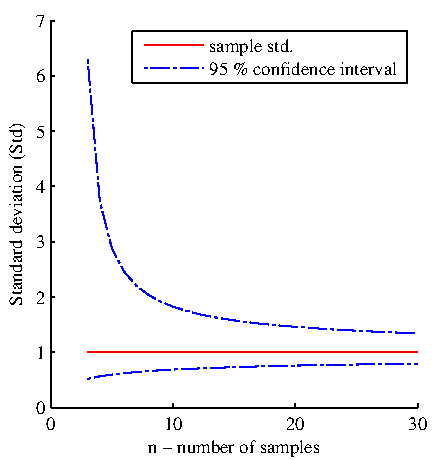
\includegraphics{stats_std_confidence.pdf}
\caption{\label{fig:std_uncertainty}Confidence interval for the population standard deviation compared to a sample standard deviation as a function of sample size. The gained certainty per measurement is best for low sample sizes.}
\end{figure}



\end{document}